% Don't touch this %%%%%%%%%%%%%%%%%%%%%%%%%%%%%%%%%%%%%%%%%%%
\documentclass[12pt]{article}
\usepackage{fullpage}
\usepackage[left=1in,top=1in,right=1in,bottom=1in,headheight=3ex,headsep=3ex]{geometry}
\usepackage{graphicx}
\usepackage{float}
\usepackage{array}


\newcommand{\blankline}{\quad\pagebreak[2]}
%%%%%%%%%%%%%%%%%%%%%%%%%%%%%%%%%%%%%%%%%%%%%%%%%%%%%%%%%%%%%%

% Modify Course title, instructor name, semester here %%%%%%%%

\title{Homework 1: Hydrostatic Fluids}
\author{PHY250 - Fall 2021}
\date{}

%%%%%%%%%%%%%%%%%%%%%%%%%%%%%%%%%%%%%%%%%%%%%%%%%%%%%%%%%%%%%%

% Don't touch this %%%%%%%%%%%%%%%%%%%%%%%%%%%%%%%%%%%%%%%%%%%
\usepackage[sc]{mathpazo}
%\linespread{1.05} % Palatino needs more leading (space between lines)
\usepackage[T1]{fontenc}
\usepackage[mmddyyyy]{datetime}% http://ctan.org/pkg/datetime
\usepackage{advdate}% http://ctan.org/pkg/advdate

\usepackage{setspace}

\newcommand{\HRule}{\rule{\linewidth}{0.5mm}}
\newdateformat{syldate}{\twodigit{\THEMONTH}/\twodigit{\THEDAY}}
\newsavebox{\MONDAY}\savebox{\MONDAY}{Mon}% Mon
\newcommand{\week}[1]{%
%  \cleardate{mydate}% Clear date
% \newdate{mydate}{\the\day}{\the\month}{\the\year}% Store date
  \paragraph*{\kern-2ex\quad #1, \syldate{\today} - \AdvanceDate[4]\syldate{\today}:}% Set heading  \quad #1
%  \setbox1=\hbox{\shortdayofweekname{\getdateday{mydate}}{\getdatemonth{mydate}}{\getdateyear{mydate}}}%
  \ifdim\wd1=\wd\MONDAY
    \AdvanceDate[7]
  \else
    \AdvanceDate[7]
  \fi%
}
%\usepackage{setspace}
\usepackage{multicol}
%\usepackage{indentfirst}
\usepackage{fancyhdr,lastpage}
\usepackage{url}
\pagestyle{fancy}
\usepackage{hyperref}
\usepackage{lastpage}
\usepackage{amsmath}
\usepackage{layout}

\lhead{}
\chead{}
%%%%%%%%%%%%%%%%%%%%%%%%%%%%%%%%%%%%%%%%%%%%%%%%%%%%%%%%%%%%%%

% Modify header here %%%%%%%%%%%%%%%%%%%%%%%%%%%%%%%%%%%%%%%%%
%\rhead{\footnotesize Text in header}

%%%%%%%%%%%%%%%%%%%%%%%%%%%%%%%%%%%%%%%%%%%%%%%%%%%%%%%%%%%%%%
% Don't touch this %%%%%%%%%%%%%%%%%%%%%%%%%%%%%%%%%%%%%%%%%%%
\lfoot{}
\cfoot{\small \thepage/\pageref*{LastPage}}
\rfoot{}

\usepackage{array, xcolor}
\usepackage{color,hyperref}
\definecolor{clemsonorange}{HTML}{EA6A20}
\hypersetup{colorlinks,breaklinks,linkcolor=clemsonorange,urlcolor=clemsonorange,anchorcolor=clemsonorange,citecolor=black}



\begin{document}


\maketitle

 \textcolor{red}{ Deadline:  09/22/2021}

\vspace{5mm}

\begin{spacing}{0.3}
    \noindent
    \HRule\\
    \HRule
\end{spacing}
\vspace{5mm}


% First Section %%%%%%%%%%%%%%%%%%%%%%%%%%%%%%%%%%%%%%%%%%%%


\newcounter{example}
\setcounter{example}{1}

\section*{Exercise \theexample \footnote{All the exercises are taken from chapter 12 of Sears and Zemansky}}

A narrow, U-shaped glass
tube with open ends is filled with
$25.0~cm$ of oil (of specific denisty
$0.80$) and $25.0 ~cm$ of water on opposite
sides, with a barrier separating
the liquids. (a) Assume
that the two liquids do not mix, and
find the final heights of the columns
of liquid in each side of the tube
after the barrier is removed. (b) For
the following cases, arrive at your
answer by simple physical reasoning,
not by calculations: (i) What would be the height on each side if the
oil and water had equal densities? (ii) What would the heights be if
the oil’s density were much less than that of water?


\begin{figure}[h!]
  \begin{center}
    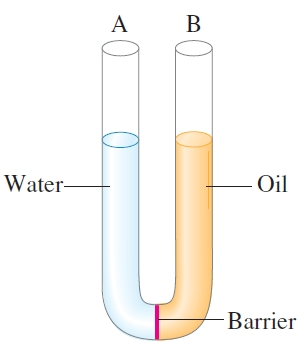
\includegraphics[height=2.6in]{images/figure4.jpg}
    \caption{Exercise \theexample }
    \label{4}
  \end{center}
\end{figure}


\stepcounter{example}
\section*{Exercise \theexample }

If the force on the
tympanic membrane (eardrum) increases by about $1.5$ N above the
force from atmospheric pressure, the membrane can be damaged.
When you go scuba diving in the ocean, below what depth could
damage to your eardrum start to occur? The eardrum is typically
$8.2$ mm in diameter. (Density of seawater: $\rho=1.03\times10^3~km/m^3$).

\stepcounter{example}
\section*{Exercise \theexample }


A cylindrical disk of
wood weighing $45.0$ N and having
a diameter of $30.0$ cm floats
on a cylinder of oil of density $0.850~g/cm^3$. The
cylinder of oil is $75.0$ cm deep
and has a diameter the same as
that of the wood. (a) What is the
gauge pressure at the top of the
oil column? (b) Suppose now
that someone puts a weight of
$83.0$ N on top of the wood, but
no oil seeps around the edge of
the wood. What is the change in
pressure at (i) the bottom of the
oil and (ii) halfway down in
the oil?



 \begin{figure}[h!]
   \begin{center}
     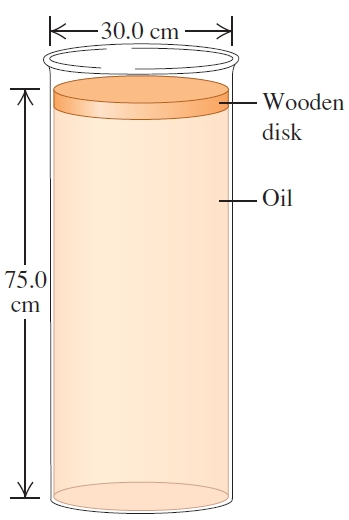
\includegraphics[height=2.4in]{images/figure1.jpg}
     \caption{Exercise \theexample }
     \label{1}
   \end{center}
 \end{figure}



 \stepcounter{example}
 \section*{Exercise \theexample  }

(a) As you can tell by watching
them in an aquarium, fish are able to remain at any depth in water
with no effort. What does this ability tell you about their density?
(b) Fish are able to inflate themselves using a sac (called the swim
bladder) located under their spinal column. These sacs can be
filled with an oxygen–nitrogen mixture that comes from the blood.
If a $2.75$-kg fish in freshwater inflates itself and increases its volume
by $10\%$, find the net force that the water exerts on it. (c) What
is the net external force on it? Does the fish go up or down when it
inflates itself?



 \stepcounter{example}
 \section*{Exercise \theexample  }
 The upper
 edge of a gate in a dam runs
 along the water surface. The
 gate is $2.00$ m high and $4.00$ m
 wide and is hinged along a horizontal
 line through its center. Calculate the
 torque about the hinge arising
 from the force due to the water.


 \begin{figure}[h!]
    \begin{center}
      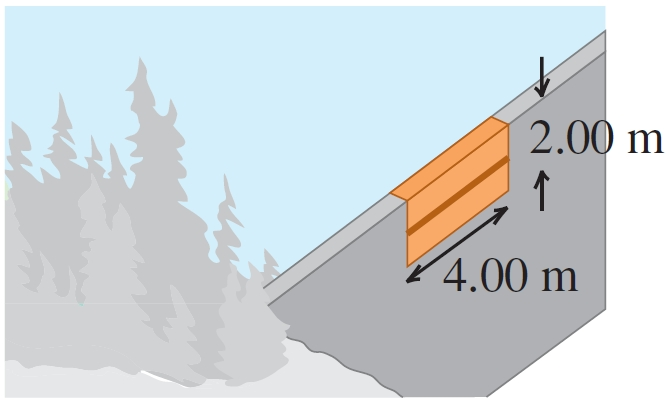
\includegraphics[height=2.4in]{images/figure3.jpg}
      \caption{Exercise \theexample }
      \label{1}
    \end{center}
  \end{figure}



 



\end{document}


